\documentclass[tikz, border=0.5mm]{standalone}
\usepackage[T1]{fontenc}
\usepackage[scaled]{beramono}
\usetikzlibrary{positioning}



\begin{document}
	
	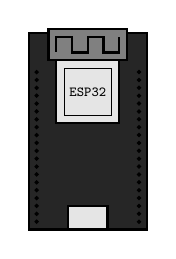
\begin{tikzpicture}[on grid,node distance=0.6cm,font=\ttfamily]
		
		%\draw[help lines,step=5mm,gray!20] (-1,-1) grid (4,4);
		
		\definecolor{LightLightGray}{rgb}{0.9,0.9,0.9}
		
		\pgfmathsetmacro{\pinDist}{0.1}
		\pgfmathsetmacro{\pinNum}{20}
		
		\tikzset{
			espAntenna/.style={
				draw,
				thick,
				fill=gray,
				minimum width=1 cm,
				minimum height=0.4 cm,
				inner sep=0,
				outer sep=0pt,
				path picture={
					\draw[thick] ++(0,0.1) -- ++(0.2,0) -- ++(0,-0.2) -- ++(0.2,0) -- ++(0,0.2);
					\draw[thick] ++(0,-0.1) -- ++(-0.2,0) -- ++(0,0.2) -- ++(-0.2,0) -- ++(0,-0.2);
					\draw[thick,cap=rect] ++(0,-0.1) -- ++(0,0.2);
				},
			},
			espSmallConn/.style={
				draw, black, thick, fill=LightLightGray,
				minimum width=0.5 cm,
				minimum height=0.3 cm,
				inner sep=0,
				outer sep=0pt,
			},
			espChip/.style={
				draw,
				thick,
				fill=LightLightGray,
				minimum size=0.8 cm,
				inner sep=0,
				outer sep=0pt,
				path picture={
					\node[draw,thin,minimum size=0.6 cm,font=\ttfamily\tiny] {ESP32};
				};
			},
			espBody/.style={
				draw, black, thick, fill=black!85,
				minimum width=1.5 cm,
				minimum height=2.5 cm,
				inner sep=0,
				outer sep=0pt,
			},
		}	
		
		
		% Body
		\node[espBody] (body) at (0,0) {};
		
		% Usb
		\node[espSmallConn,above=0cm of body.south] (usb) {};
		
		% Connector
		\foreach \i in {1,...,\pinNum} {
			\filldraw (body.south west) ++ (0.1,\i*\pinDist) circle (0.02);
			\filldraw (body.south east) ++ (-0.1,\i*\pinDist) circle (0.02);
		}
		
		% Wi-Fi
		\node[espChip] (esp32) at (0,0.5) {};
		
		% Antenna
		\node[espAntenna,above=0cm of esp32.north] (antenna) {};
		
		
		% Logo
		%\node at (1,1.5) {\includegraphics[width=0.6cm]{logo_raspberry.pdf}};
		
		
	\end{tikzpicture}
\end{document}
